% Exemplo de relatório técnico do IC
% Criado por P.J.de Rezende antes do Alvorecer da História.
% Modificado em 97-06-15 e 01-02-26 por J.Stolfi.
% Last edited on 2003-06-07 21:12:18 by stolfi
% modificado em 1o. de outubro de 2008
% modificado em 2012-09-25 para ajustar o pacote UTF8. Contribuicao de
%   Rogerio Cardoso

\documentclass[11pt,twoside]{article}
\usepackage{techrep-ic}
\usepackage{indentfirst}

%%% SE USAR INGLÊS, TROQUE AS ATIVAÇÕES DOS DOIS COMANDOS A SEGUIR:
\usepackage[brazil]{babel}
%% \usepackage[english]{babel}

%%% SE USAR CODIFICAÇÃO LATIN1, TROQUE AS ATIVAÇÕES DOS DOIS COMANDOS A
%%% SEGUIR:
%% \usepackage[latin1]{inputenc}
\usepackage[utf8]{inputenc}
\usepackage{graphicx}
\usepackage{url}
\begin{document}

%%% PÁGINA DE CAPA %%%%%%%%%%%%%%%%%%%%%%%%%%%%%%%%%%%%%%%%%%%%%%%
%
% Número do relatório
\TRNumber{03}

% DATA DE PUBLICAÇÃO (PARA A CAPA)
%
\TRYear{16}  % Dois dígitos apenas
\TRMonth{06} % Numérico, 01-12

% LISTA DE AUTORES PARA CAPA (sem afiliações).
\TRAuthor{Gabriel Oliveira \and Jo{\~a}o Fid{\'e}lis \and Lucas Morais \and Matheus Figueiredo \and Pedro Grij{\'o}}

% TÍTULO PARA A CAPA (use \\ para forçar quebras de linha).
\TRTitle{MC437 - Grupo06 - Relat{\'o}rio 3}

\TRMakeCover
%%%%%%%%%%%%%%%%%%%%%%%%%%%%%%%%%%%%%%%%%%%%%%%%%%%%%%%%%%%%%%%%%%%%%%
% O que segue é apenas uma sugestão - sinta-se à vontade para
% usar seu formato predileto, desde que as margens tenham pelo
% menos 25mm nos quatro lados, e o tamanho do fonte seja pelo menos
% 11pt. Certifique-se também de que o título e lista de autores
% estão reproduzidos na íntegra na página 1, a primeira depois da
% página de capa.
%%%%%%%%%%%%%%%%%%%%%%%%%%%%%%%%%%%%%%%%%%%%%%%%%%%%%%%%%%%%%%%%%%%%%%

%%%%%%%%%%%%%%%%%%%%%%%%%%%%%%%%%%%%%%%%%%%%%%%%%%%%%%%%%%%%%%%%%%%%%%
% Nomes de autores ABREVIADOS e titulo ABREVIADO,
% para cabeçalhos em cada página.
%
\markboth{Bueno, Fid{\'e}lis, Figueiredo, Grij{\'o}, Morais}{MC437 - Grupo06}
\pagestyle{myheadings}

%%%%%%%%%%%%%%%%%%%%%%%%%%%%%%%%%%%%%%%%%%%%%%%%%%%%%%%%%%%%%%%%%%%%%%
% TÍTULO e NOMES DOS AUTORES, completos, para a página 1.
% Use "\\" para quebrar linhas, "\and" para separar autores.
%
\title{MC437 - Grupo06}

\author{Gabriel Bueno de Oliveira \and
Jo{\~a}o Guilherme Daros Fid{\'e}lis \and
Lucas Henrique Morais \and
Matheus Yokoyama Figueiredo \and Pedro Rodrigues Grij{\'o}}
\date{}

\maketitle

%%%%%%%%%%%%%%%%%%%%%%%%%%%%%%%%%%%%%%%%%%%%%%%%%%%%%%%%%%%%%%%%%%%%%%

\begin{abstract}
\setlength{\parindent}{4ex}
Este é o relat\'orio final do projeto da disciplina MC437 (Projeto de Sistemas de Informa\c{c}\~ao), projeto cujo objetivo foi a resolução de um problema de replicação de banco de dados. Foram utilizados dois bancos de dados diferentes, um atuando como primário e outro como secundário. O primário é replicado para um secundário em hot-standby. Ao inserirmos uma falha, promovemos o secundário para primário e fazemos o antigo primário voltar como secundário, sendo que o objetivo foi obter o menor tempo de indisponibilidade possível no sistema.
Utilizamos o benchmark TPC-W, que modela uma livraria online, atrav\'es de um ambiente controlado, para simular atividades num servidor WEB. Em conjunto com o simulador RBE, que gera tr\^es diferentes perfis de carga (Shopping, Ordering e Browsing), pudemos checar o desempenho do servidor instalado num cluster no IC, ao verificarmos o n\'umero de WIPS (WEB Interactions per Second) e WIRT (WEB Interaction Response Time) gerados por diferentes cargas.
\end{abstract}

\section{Introdução}


Este \'e o relat\'orio final do projeto da disciplina MC437 - Projeto de Sistemas de Informação. O objetivo do projeto foi a definição e implementação de uma solução para o problema de replicação de banco de dados. As cargas de trabalho utilizadas para testar a solução de replicação foram geradas por uma implementação do Transaction Processing Council-Web Benchmark (TPC-W)~\cite{TPCW}. A meta final foi obter um sistema com a maior disponibilidade (1) e desempenho (2) possíveis. 

\begin{equation} \label{eq:1}
a = \frac{tempo\_em\_operacao}{tempo\_em\_operacao + tempo\_inoperante}
\end{equation}

\begin{equation} \label{eq:2}
d = web\_interactions\_per\_second(WIPS)
\end{equation}

Onde tempo\_em\_operação é o período de tempo em que o sistema
está apto a responder requisições de seus usuários, tempo\_inoperante é o período de tempo em que o sistema é incapaz de
produzir respostas corretas para as requisições realizadas pelos
usuários e, finalmente, web\_interactions\_per\_second é o número de requisições web por segundo que ocorrem no sistema. Num sistema ideal, a = 1 e d \rightarrow \infty.

Durante a elaboração do projeto, foram implementadas e testadas maneiras de recuperação em caso de falhas num banco de dados. A disponibilidade, dada pela equação (1), indica que o tempo em que o sistema fica inoperante deve ser o menor possível para que essa seja alta.

Para isso foi aplicada a técnica de Streaming Replication~\cite{SR}, na qual um banco de dados é mantido como primário, recebendo operações de leitura e escrita. Para garantir alta disponibilidade, foi utilizada redundância, mantendo outro banco de dados (em outra máquina) como secundário em hot-standby. Um banco em hot-standby nada mais é do que uma cópia "quente" do banco primário que só faz operações de leitura, de forma que caso o primário seja desligado, o secundário possa ser promovido a primário (passando a permitir também operações de escrita) imediatamente, mantendo o sistema num estado consistente. O Streaming Replication garante que toda operação de escrita feita no banco primário seja repassada e feita também no secundário, para que este possa ser promovido imediatamente, caso necessário. Esta técnica permite que muitos bancos fiquem em standby, garantindo alta disponibilidade e confiablidade ao sistema. No caso deste projeto, foram empregados apenas um banco primário e um banco secundário nos experimentos.

O projeto foi dividido em 3 arcos de desenvolvimento, explicados brevemente a seguir.

\subsection{Arco de desenvolvimento 01}

    No primeiro arco o objetivo foi a configuração do sistema inicial para testar o desempenho e a disponibilidade do mesmo. Não ocorreu injeção de falhas no sistema, apenas foi variada a quantidade de clientes para que fosse obtido um número ideal de WIPS (alto, que não deixe o sistema indisponível) para os próximos testes.

\subsection{Arco de desenvolvimento 02}

    O segundo arco parte dos resultados obtidos no arco 01. A diferença está na injeção de falha. Aqui foram feitos 3 experimentos para medir desempenho e disponibilidade, caracterizados a seguir: 
    \begin{itemize}
        \item Apenas com o banco primário funcionando.
        \item Bancos primário e secundário funcionando.
        \item Bancos primário e secundário funcionando, injeção de falha no primário e promoção do banco secundário para primário automaticamente.
    \end{itemize}

\subsection{Arco de desenvolvimento 03}

    O terceiro e último arco segue dos resultados obtidos no arco 02. Aqui o diferencial são a detecção de falhas e a promoção automática do banco secundário para primário (e vice-versa) quando necessário. A seguir, este relatório discorre sobre as condições experimentais, metodologia de pesquisa e resultados obtidos neste arco final.

\setlength{\parindent}{4ex}


\section{Condições Experimentais}
\setlength{\parindent}{4ex}
     Nesta se\c{c}\~ao ser\~ao descritas as configura\c{c}\~oes de hardware e software utilizadas nos experimentos.

\subsection{Plataforma de Testes}

     Nesta fase do trabalho contamos com quatro máquinas fornecidas pelo Instituto de Computação. As máquinas são iguais do ponto de vista de configuração de hardware, e esta pode ser observada na Tabela 1.
     
    \begin{center}
        \begin{tabular} { | c || c |}
        \hline
        Sistema Operacional & Ubuntu 14.04 \\ \hline
        CPU & Intel(R) Core(TM)2 Quad CPU Q8400 2.66GHz \\ \hline
        Memória RAM & 4GB e 1333 MHz de frequência \\ 
        \hline
        \end{tabular}
        %\caption{\label{tab:tableOne}Configurações das máquinas remotas}

        Tabela 1: Configuração das máquinas remotas
    \end{center}

\subsection{Arquitetura de Software da Solução}

    A distribuição dos programas utilizados na solução foi feita conforme consta na Tabela 2.

    \begin{center}
        \begin{tabular}{| c | c | c | c |}
            \hline
            \multicolumn{4}{|c|}{Máquinas} \\ \hline
            \textbf{CBN6} & \textbf{CBN7} & \textbf{dbmaster2} & \textbf{dbslave2} \\ \hline
            HAProxy 1.6 & RBE & PostgreSQL 9.5.1 & PostgreSQL 9.5.1 \\ \hline
            Apache Tomcat 7 & - & - & - \\ \hline
            TPC-W & - & - & - \\ \hline
        \end{tabular}
        
        Tabela 2: Softwares em cada máquina do cluster
    \end{center}

    A \textbf{CBN6} atua como servidor web. Nela foi instalado um servidor Apache Tomcat~\cite{tomcat} e o aplicativo TPC-W, um benchmark de transa\c{c}\~oes web que implementa uma livraria digital. 
    
    Para fazer uso do TPC-W foi utilizado o RBE (Remote Browser Emulator)~\cite{RBE}, que foi colocado separadamente na \textbf{CBN7}. O RBE \'e um simulador, escrito completamente em Java, que simula o tr\'afego HTTP gerado por um usu\'ario que estivesse acessando o site atrav\'es de um navegador. Neste trabalho, sua função foi de emular os conjuntos de clientes que acessam o lado servidor do TPC-W. O motivo que levou à instalação do RBE em uma máquina separada do servidor foi tentar obter um melhor desempenho nos testes, pois desse modo o trabalho ficou dividido entre 4 máquinas ao invés de apenas 3. 

    Também na \textbf{CBN6} foi colocado o HAProxy~\cite{haproxy}, que atua como um proxy para aplicações baseadas em TCP e HTTP. Ele oferece alta disponibilidade e balanceamento de carga para servidores web. 
    
    Nas outras duas máquinas remotas foram instaladas instâncias de bancos de dados PostgreSQL~\cite{postgresql}, uma com um banco atuando como primário (\textbf{dbmaster2}) e outra com um banco secundário (\textbf{dslave2}) inicialmente em hot-standby. Assim, o HAProxy foi utilizado para detectar falha do banco primário e redirecionar as requisições feitas para o banco secundário, que deve ser promovido a banco primário.
    
    Ao integrarmos essas funcionalidades, conseguimos emular um site de compras com dados gerados aleatoriamente.

    O TPC-W gera as duas métricas em que nos baseamos para avaliar o desempenho do sistema: WIPS (Web Interactions per Second) e WIRT (Web Interaction Response Time). A carga de trabalho gerada pelo RBE pode ser de tr\^es perfis: \textit{shopping}(WIPS), \textit{browsing}(WIPSb) ou \textit{ordering}(WIPSo). Cada perfil corresponde a uma porcentagem diferente de operações de leitura e escrita no banco de dados, como exemplificado na Tabela 3.

        \begin{center}
        \begin{tabular} { | c | c | c |}
        \hline
        Perfil  & Leitura & Escrita \\ \hline
        WIPSb & 95\% & 5\% \\ \hline
        WIPS & 80\% & 20\% \\ \hline
        WIPSo & 50\% & 50\% \\
        \hline
        \end{tabular}
        %\caption{\label{tab:tableOne}Configurações das máquinas remotas}

        Tabela 3: Descrição das operações dos perfis do RBE
    \end{center}


    Rodamos o RBE com os três perfis variando o parâmetro Think-Time. O Think-Time é o tempo que um usuário simulado pelo RBE gasta "pensando", ou seja, quanto menor o Think-Time, mais requisições são enviadas ao servidor pelos usuários no mesmo período de tempo de experimento.

\section{Metodologia de Pesquisa}
\setlength{\parindent}{4ex}
Após todo o sistema estar rodando de maneira estável, objetivo atingido no primeiro arco, foram realizados experimentos no segundo arco para determinar uma carga que o sistema conseguisse atender. No primeiro experimento, o RBE foi utilizado com apenas o banco primário ligado. No segundo, estavam ligados o banco primário e o banco secundário em hot-standby.

Esses dois experimentos foram realizados para caracterizar o servidor. O objetivo foi medir a maior carga para a qual ele se comportasse de forma consistente. Para isso, os valores de carga foram variados entre 2000 e 4000 clientes, variando de 1000 em 1000 para cada iteração para cada perfil de usuário descrito na Tabela 3. Assim,  gráficos foram gerados para demonstrar até qual carga o servidor se manteve num bom nível de WIPS ao longo de todo o teste (que dura 100s no total).

O valor encontrado foi utilizado no RBE para simular essa "carga ótima" no servidor, causando uma falha manualmente (isto é, "matando" o banco de dados primário), enquanto o banco de dados secundário era promovido. O objetivo foi checar em quanto tempo o servidor conseguiria se recuperar e voltar a ficar ativo.

Os parâmetros utilizados no RBE foram:

    \begin{center}
        \begin{tabular} { | c | c | c |}
        \hline
        Ramp-Up  & 5s \\ \hline
        Ramp-down & 5s \\ \hline
        Measurement Interval & 90s \\ \hline
        Número máximo de erros & 0 \\ \hline
        Think-Time & 1s \\
        \hline
        \end{tabular}
        %\caption{\label{tab:tableOne}Configurações das máquinas remotas}

        Tabela 4: Parâmetros dos experimentos do RBE
    \end{center}
    

Após o estudo do comportamento do servidor perante variações de carga, foi observado que a diminuiição do Think-Time levava à instabilidade do sistema, mesmo com a "carga ótima" encontrada anteriormente.

Devido a isso, no terceiro arco foi decidido que seria aplicada metade da "carga ótima" para os próximos passos, pois partindo de um valor de Think-Time igual a metade do valor utilizado anteriormente (de 1s para 0.5s), o número de requisições feitas seria o mesmo. 

O último experimento, o completo, consistiu na inserção de uma falha na \textbf{dbmaster2}. Essa máquina, inicialmente contendo o banco primário, era então substituída pela \textbf{dbslave2}, ou seja, \textbf{dbslave2} era promovida a banco primário. Após a \textbf{dbmaster2} se recuperar, esta  voltava como banco secundário. Depois de alguns segundos, uma outra falha era inserida, agora na \textbf{dbslave2}, que após sua queda era substituída pela \textbf{dbmaster2} ( promovida à banco primário) e, finalmente, após se recuperar a \textbf{dbslave2} voltava como banco secundário, como no início do experimeno.

Para inserir as falhas, foi utilizado o comando stop do PostgreSQL para parar o banco de dados. Quando a falha ocorre, o HAProxy começa a redirecionar as requisições do banco primário para o banco secundário, que por sua vez está sendo promovido à primário por um script. Ao mesmo tempo, um outro script foi utilizado para checar o status dos bancos de dados. Ao detectar que um deles falhou, o script muda o arquivo de configuração do HAProxy para informar ao programa qual o novo banco de dados primário e qual o novo secundário. O banco de dados que foi derrubado é religado, agora como banco secundário. Isso pode acontecer quantas vezes forem necessárias. No experimento realizado, cada banco é pelo menos uma vez o banco primário e é derrubado para retornar como secundário.

Assim, com carga de 1000 usuários, o Think-Time foi variado de 0.5s a 0.1s. Isso quer dizer que seriam feitas muito mais requisições que a mesma carga sendo aplicada com 2000 usuários e Think-Time de 1s.

\section{An\'alise e Resultados}
\setlength{\parindent}{4ex}

Seguem os gráficos gerados pela execução do RBE para o experimento 1.
\begin{center}
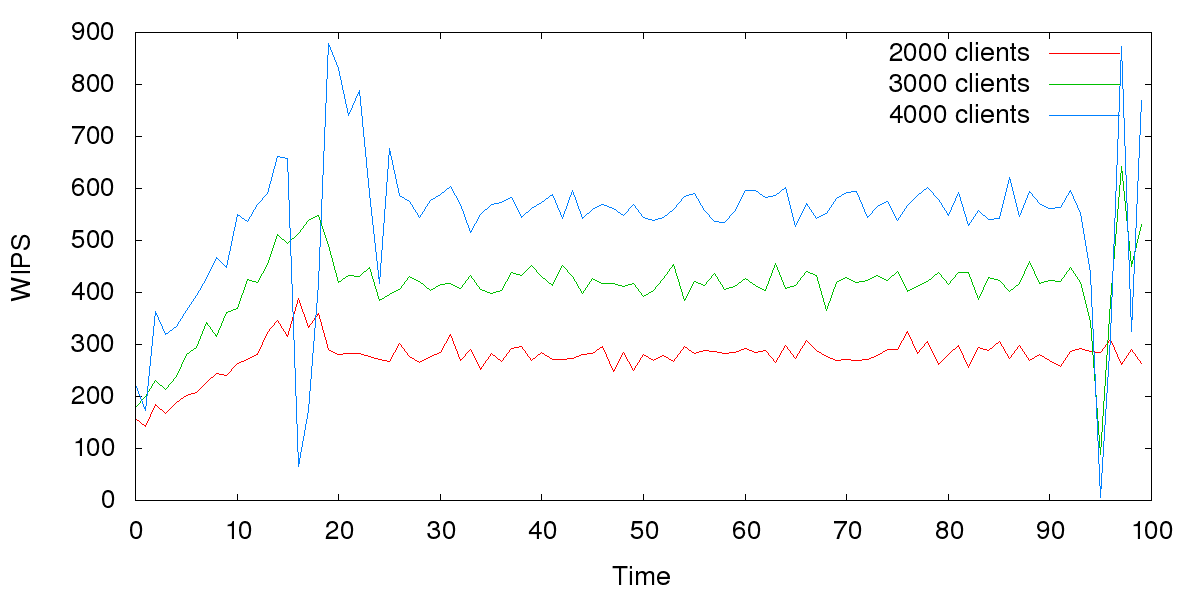
\includegraphics[width=15cm, height=10cm]{images/exp1/plot_browsin}
Figura 1: WIPSb por tempo(s) para cada carga simulada pelo RBE no perfil Browsing do experimento 1
\end{center}
Nota-se que o experimento com 4000 clientes teve uma boa consistência entre 30 e 90 segundos, porém houve uma grande queda por volta dos 15s e a partir dos 90s. O mesmo ocorreu no caso para 3000 clientes a partir de 90s.

\begin{center}
\vspace{-1em}
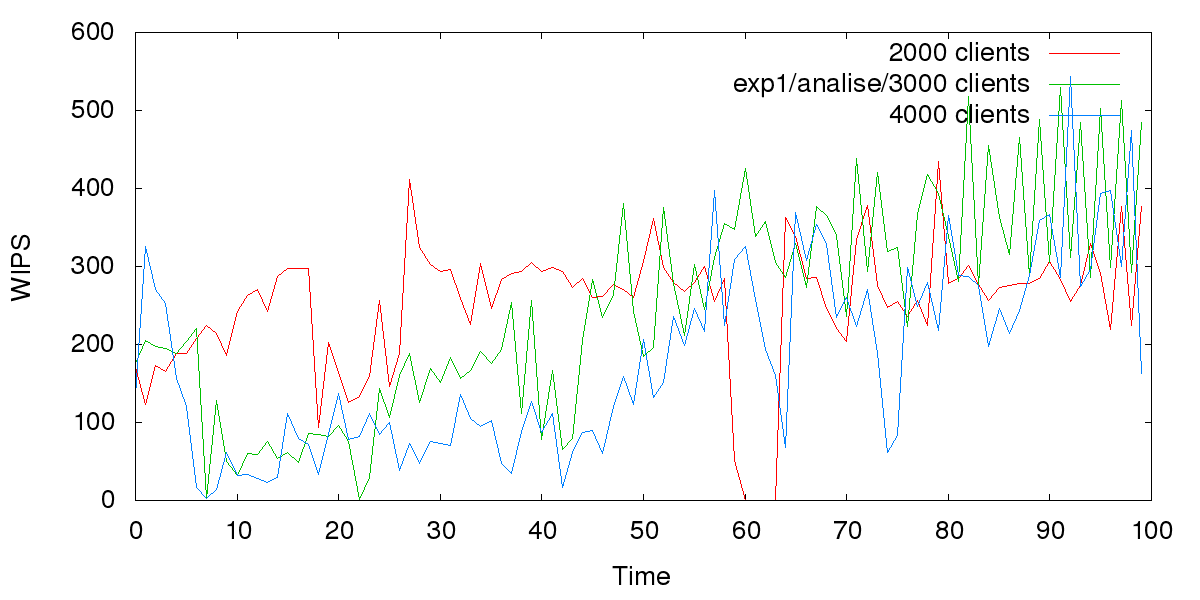
\includegraphics[width=15cm, height=10cm]{images/exp1/plot_ordering}
Figura 2: WIPSo por tempo(s) para cada carga simulada pelo RBE no perfil Ordering do experimento 1
\end{center}
Pelo gráfico, é visível que o teste com 3000 clientes obteve o melhor desempenho no geral. Até 50s, o desempenho era melhor com 2000 clientes, porém após esse tempo o teste com 3000 clientes obteve uma quantidade maior de WIPSo e se manteve consistentemente melhor que os testes com 2000 e 4000 clientes.

\begin{center}
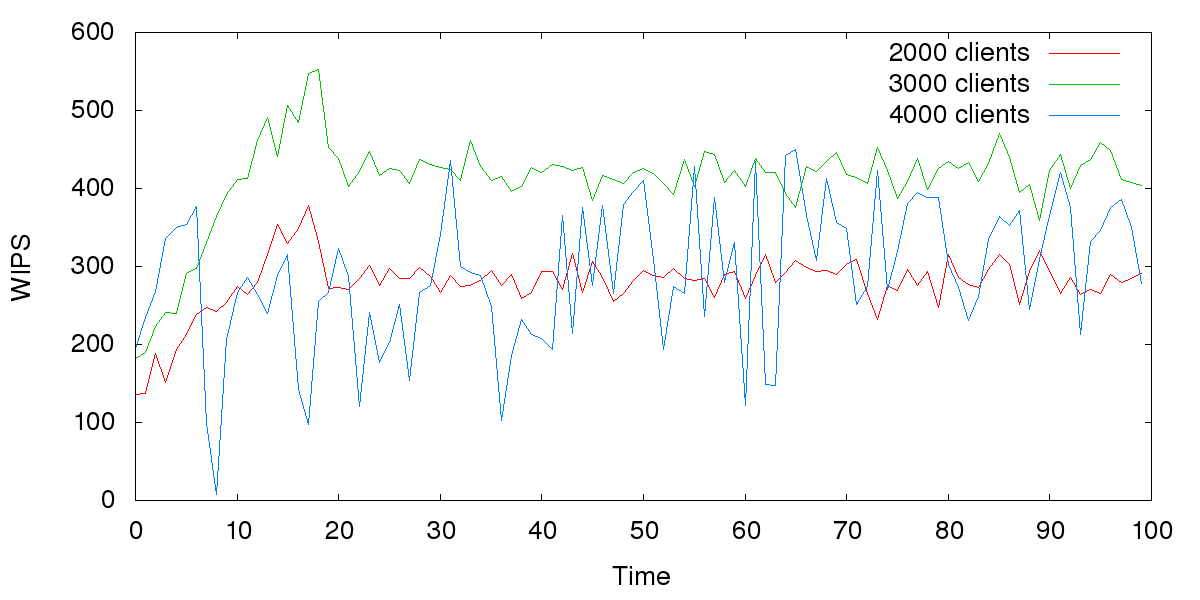
\includegraphics[width=15cm, height=10cm]{images/exp1/plot_shopping}
Figura 3: WIPS por tempo(s) para cada carga simulada pelo RBE no perfil Shopping do experimento 1
\end{center}

Neste gráfico, ficou evidente o melhor desempenho da simulação com 3000 clientes sobre as duas outras. Uma melhor taxa de WIPS foi obtida durante praticamente todo o experimento.

Com a combinação dos resultados desses gráficos, temos indícios de que 3000 usuários talvez seja o melhor número a ser utilizado, pois tem taxas de WIPS mais altas e estáveis que as outras quantidades de usuários testadas.

Agora, analisaremos os dados do experimento 2.

\begin{center}
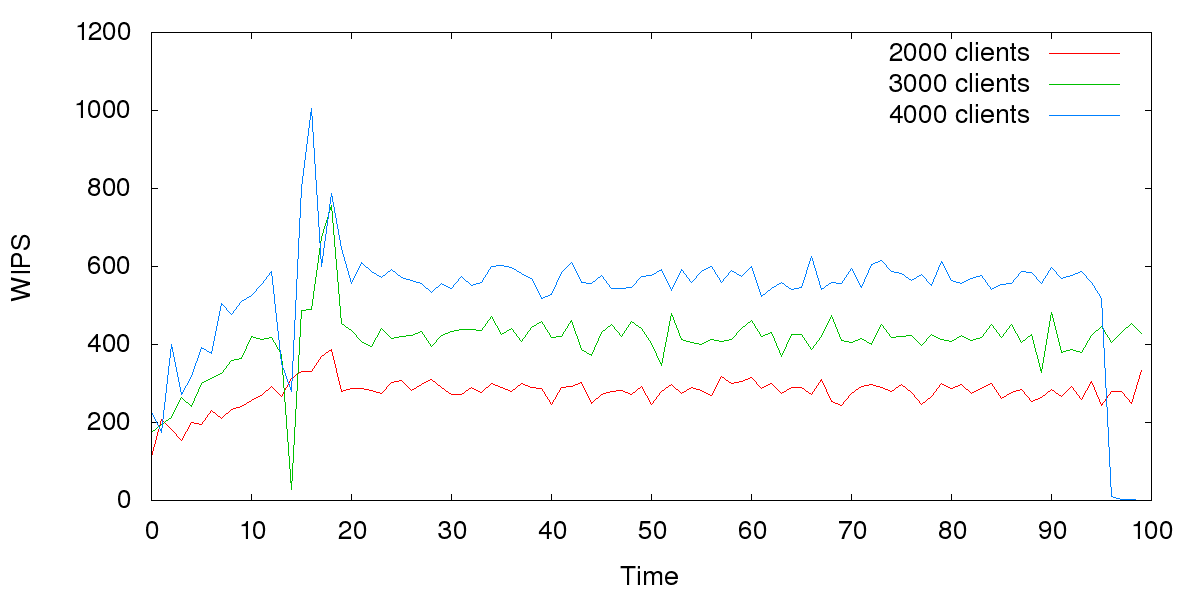
\includegraphics[width=15cm, height=10cm]{images/exp2/plot_browsin}
Figura 4: WIPSb por tempo(s) para cada carga simulada pelo RBE no perfil Browsing do experimento 2
\end{center}

O gráfico indica um melhor desempenho geral para 4000 clientes. Entretanto, no final do experimento há uma grande queda, que indica problemas devido a alta carga. Nesse caso, 3000 clientes apresenta melhor estabilidade em relação a 4000 e maior quantidade de WIPSb em relação a 2000 clientes

\begin{center}
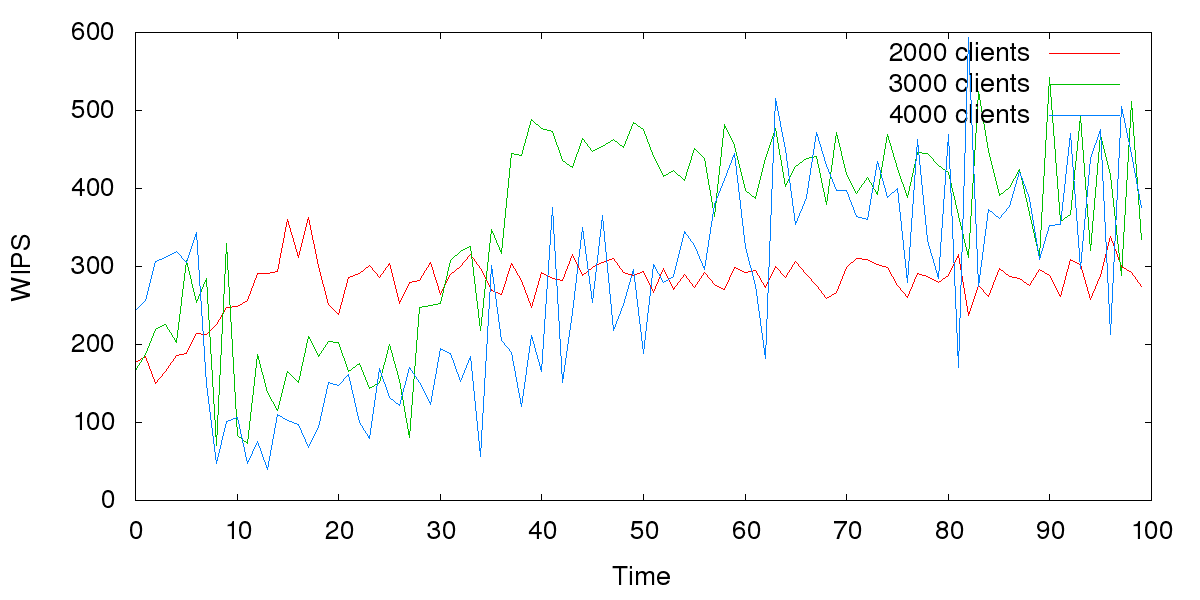
\includegraphics[width=15cm, height=10cm]{images/exp2/plot_ordering}
Figura 5: WIPSo por tempo(s) para cada carga simulada pelo RBE no perfil Ordering do experimento 2
\end{center}

O melhor desempenho geral foi para 3000 clientes, pois essa carga manteve uma boa média durante todo o experimento e se manteve no mesmo nível de WIPSo para 4000 clientes na segunda metade do experimento.

\begin{center}
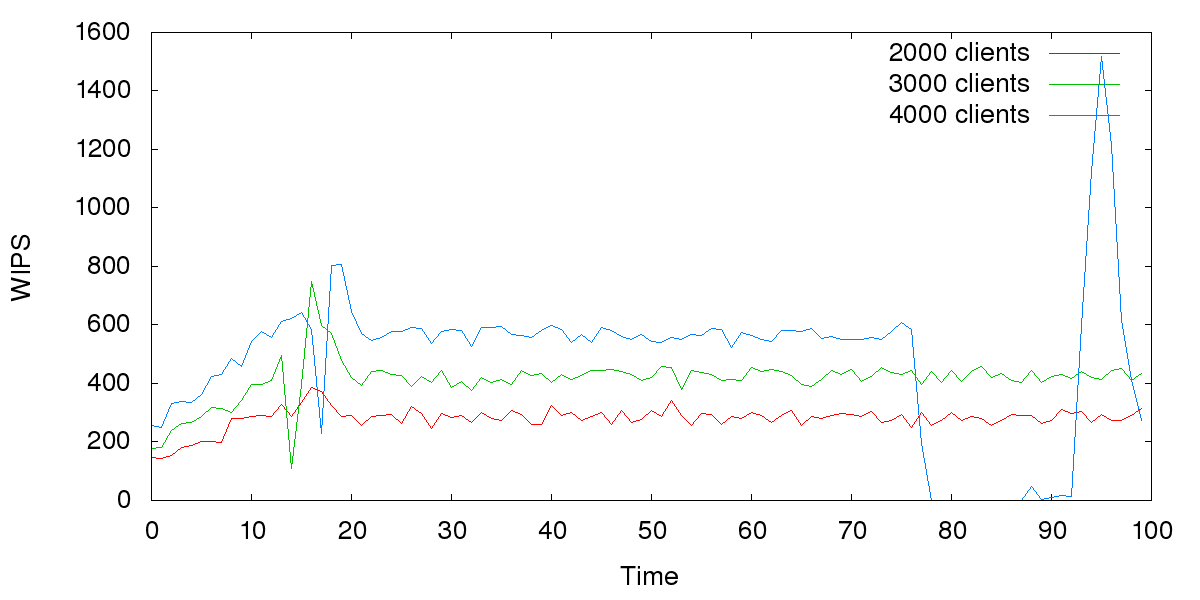
\includegraphics[width=15cm, height=10cm]{images/exp2/plot_shopping}
Figura 6: WIPS por tempo(s) para cada carga simulada pelo RBE no perfil Shopping do experimento 2
\end{center}

Este resultado se assemelha ao do perfil Browsing. 4000 clientes possui bom desempenho até aproximadamente 70s do experimento, quando sofre queda de WIPS, o que indica que está alta carga sobrecarrega o servidor. Como no perfil Browsing, a carga mais estável é de 3000 clientes.

Definimos então rodar o experimento três (com failover) utilizando uma carga de 3000 clientes.

\begin{center}
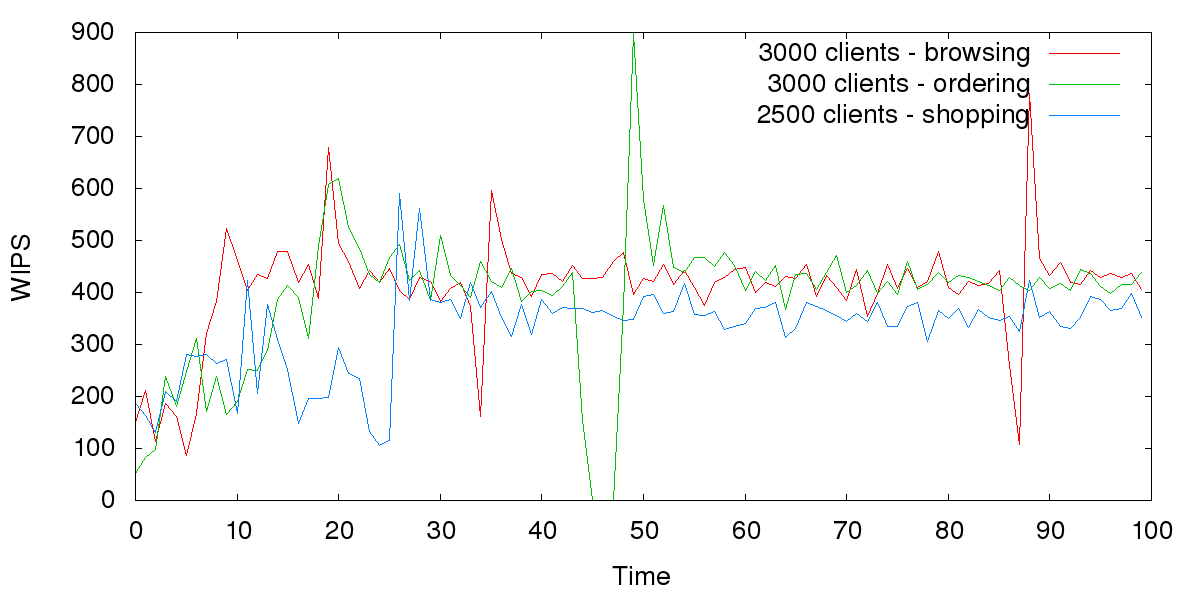
\includegraphics[width=15cm, height=10cm]{images/exp3/plot_exp3}
Figura 7: WIPS por tempo(s) para cada perfil simulado pelo RBE no experimento 3
\end{center}

Este gráfico indicas alguns resultados interessantes. Podemos ver que não houve queda de desempenho nos perfis de browsing e shopping, mesmo após a falha. Isso ocorreu provavelmente pois nosso script finaliza o processo do banco de dados primário (causando a falha) e logo em seguida já promove o secundário que rapidamente assume como primário, pois o HAProxy é rápido em notar que o primário falhou e já redireciona as requisições para o secundário.
Porém, notamos que no perfil Ordering, onde tem muito mais instruções de escrita, que são muito custosas, a carga de 3000 causou falhas no servidor. Portanto, utilizamos uma carga de 2500 e conseguimos resultados satisfatórios. Vemos que a falha ocorre perto da marca de 45s e que o servidor se recupera por volta de 49s, o que equivale a um pouco menos de quatro segundos de recuperação.

Com esses dados, definimos uma carga ótima de 2000 clientes (com Think-Time = 1s), pois é um pouco abaixo dos 2500 clientes testados acima, deixando uma margem de segurança. A partir disso, começamos a variar o Think-Time e a realizarmos o experimento completo, alternando os bancos de dados múltiplas vezes entre primário e secundário. Utilizamos metade dos clientes, ou seja, 1000 clientes, pois iniciamos o Think-Time com metade do seu valor inicial.

\begin{center}
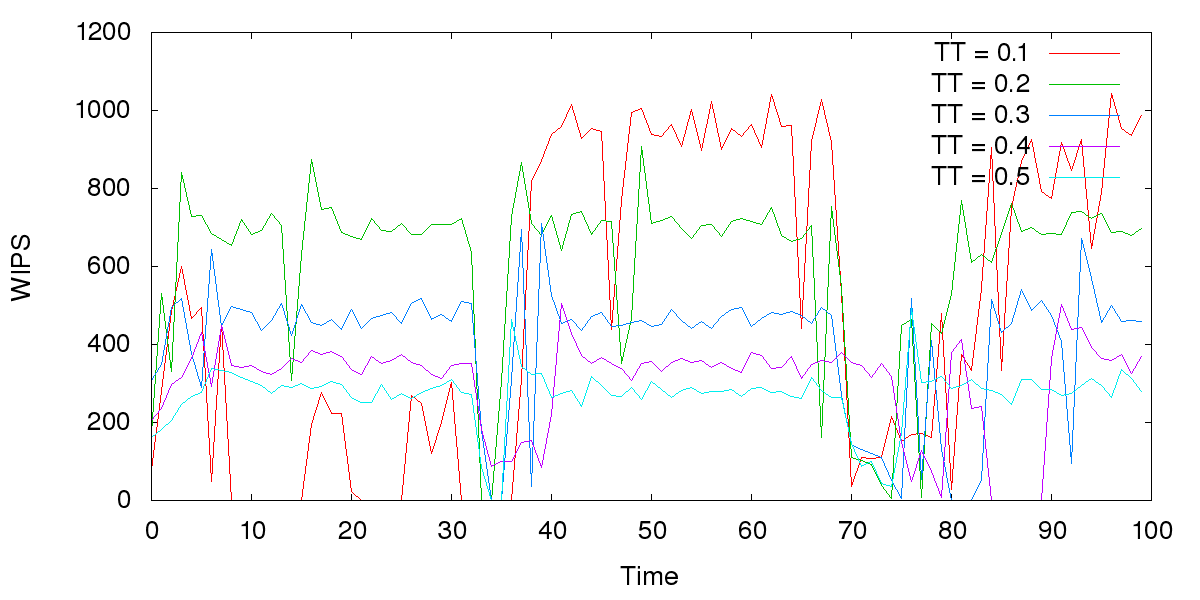
\includegraphics[width=15cm, height=10cm]{images/completo/plot_browsing.png}
Figura 8: WIPSb por tempo(s) para cada Think-Time testado no perfil de Browsing no experimento completo
\end{center}

Vemos que para Think-Time muito baixos o WIPSb foi bem inconsistente, próximo de 0 nos primeiros 30s de experimento. Nota-se claramente os pontos onde as falhas nos primários foram inseridas pela queda de WIPSb para zero por um período. Os valores que mostraram melhor desempenho e estabilidade foram Think-Time de 0.2s e 0.3s.

\begin{center}
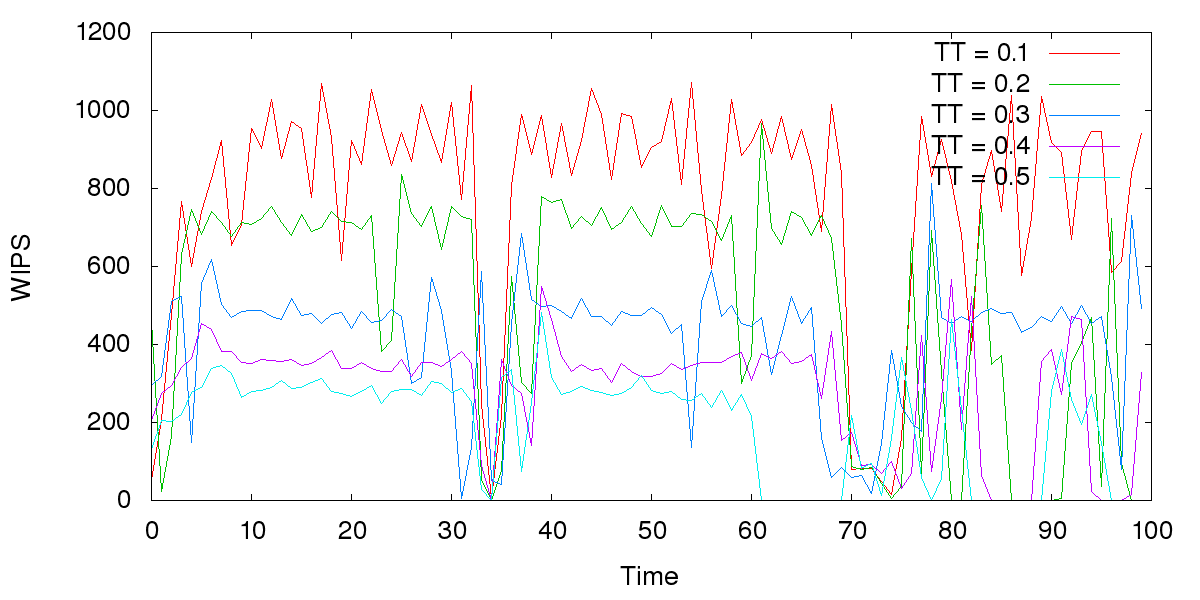
\includegraphics[width=15cm, height=10cm]{images/completo/plot_shopping.png}
Figura 9: WIPS por tempo(s) para cada Think-Time testado no perfil de Shopping no experimento completo
\end{center}

O gráfico se manteve mais consistente, podendo ver a queda do banco de dados primário perto dos 30s e depois, novamente, perto dos 70s.  Os melhores desempenhos foram obtidos pelos Think-times mais baixos.

\begin{center}
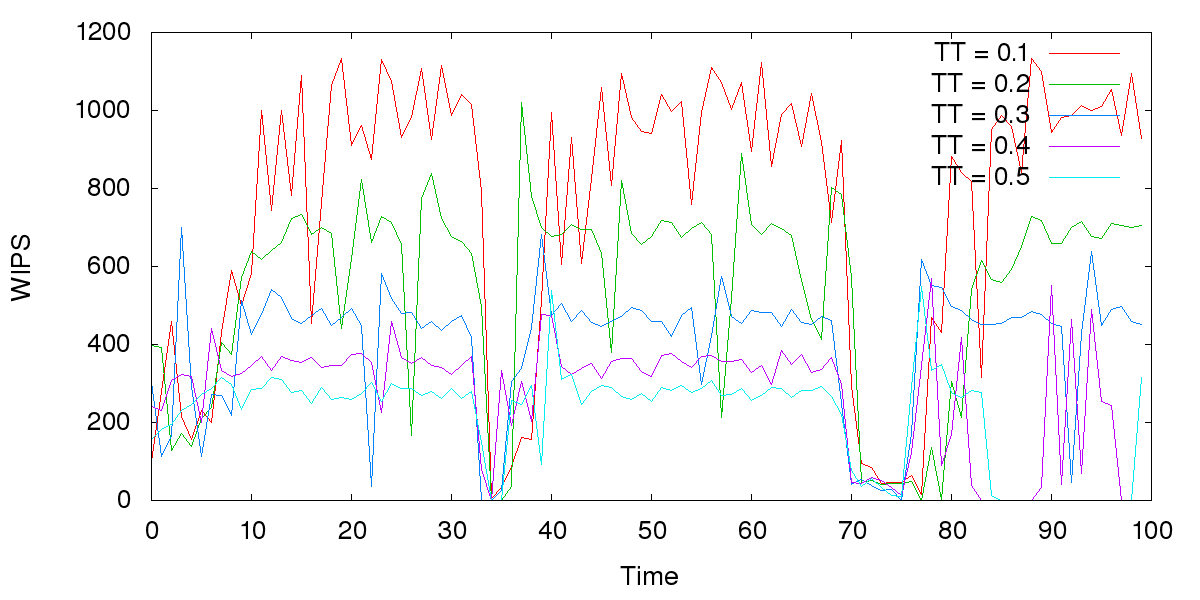
\includegraphics[width=15cm, height=10cm]{images/completo/plot_ordering.png}
Figura 10: WIPSo por tempo(s) para cada Think-Time testado no perfil de Ordering no experimento completo
\end{center}

O gráfico também se manteve consistente, podendo ver a queda do banco de dados primário perto dos 30s e depois, novamente, perto dos 70s.  Os melhores desempenhos foram obtidos pelos Think-Times mais baixos, novamente.

Analisando esses três gráficos, vemos que um valor estável e com bom desempenho foi o de Think-Time de 0.3s.

Para melhor ilustrar nossos resultados, fizemos gráficos com apenas os dados de Think-Time de 0.3s com 1000 clientes para os três perfis.

\begin{center}
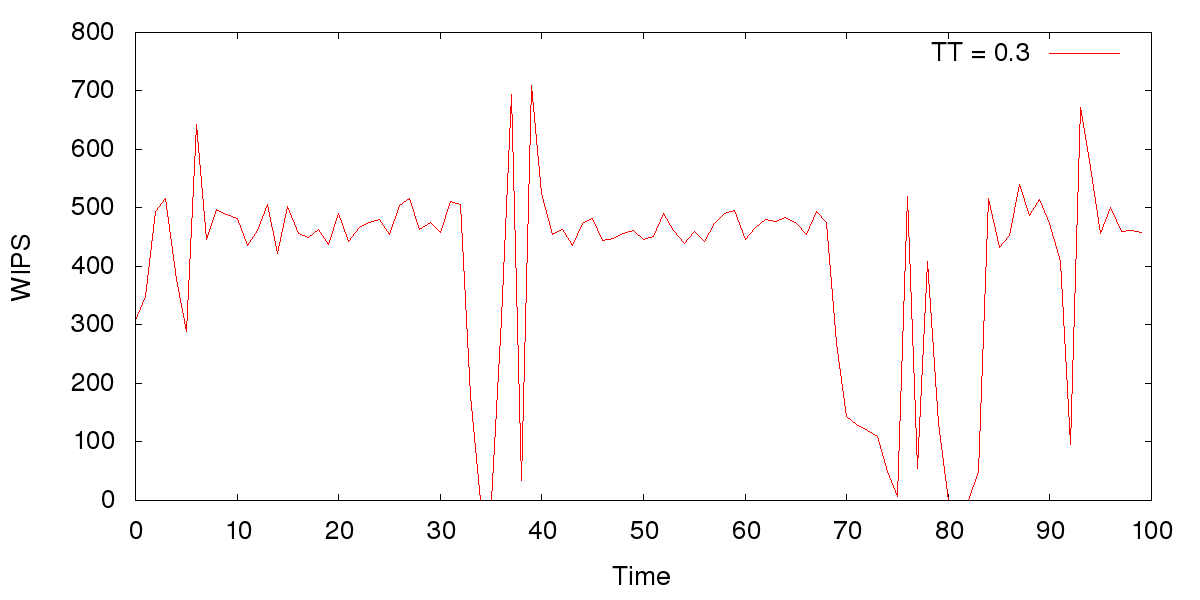
\includegraphics[width=15cm, height=10cm]{images/completo/plot_browsing_TT03.png}
Figura 11: WIPSb por tempo(s) para Think-Time de 0.3s testado no perfil de Browsing no experimento completo
\end{center}

Pelo gráfico, vemos que após a primeira queda, por volta de 32s, o sistema voltou a ficar estável próximo aos 40s. A segunda queda ocorreu perto dos 68s e voltou à estabilidade perto dos 84s. Temos um tempo inoperante total de 24s e tempo de operação de 76s. Pela equação (1), nossa disponibilidade ficou por volta de 76\%.

\begin{center}
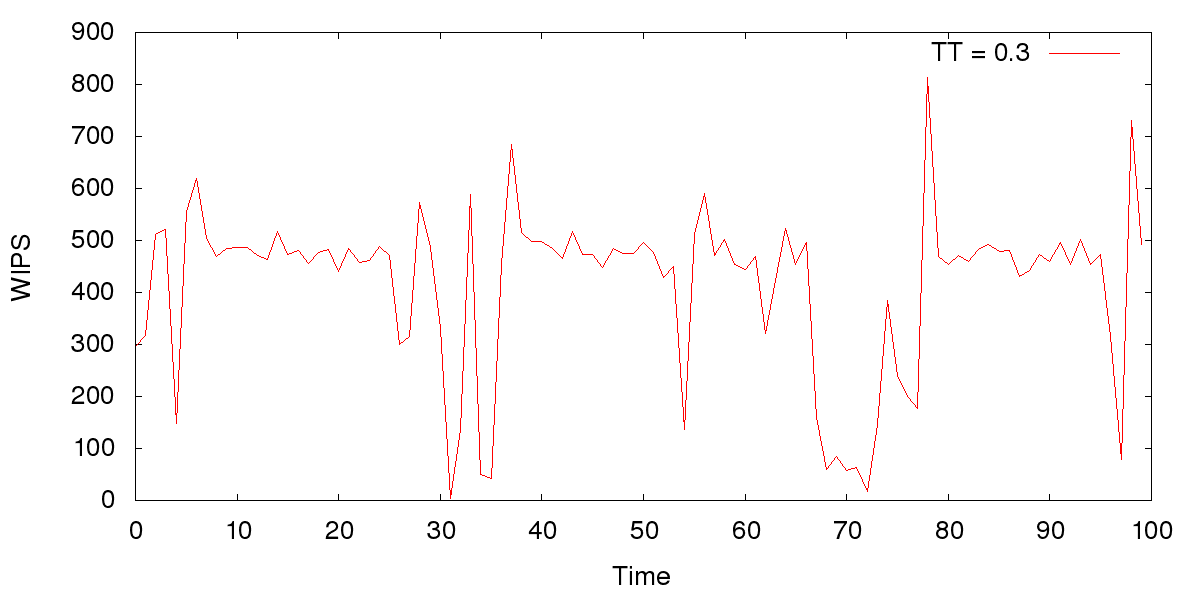
\includegraphics[width=15cm, height=10cm]{images/completo/plot_shopping_TT03.png}
Figura 12: WIPS por tempo(s) para Think-Time de 0.3s testado no perfil de Shopping no experimento completo
\end{center}

Novamente, a primeira queda ocorreu por volta de 29s e se recuperou totalmente perto dos 37s. Já a segunda queda ocorreu próxima aos 65s e a recuperação ocorreu em 78s. O tempo inoperante ficou em torno de 21s e o tempo operante em 79s. Portanto, pela equação (1), o a disponibilidade ficou em torno de 79\%.

\begin{center}
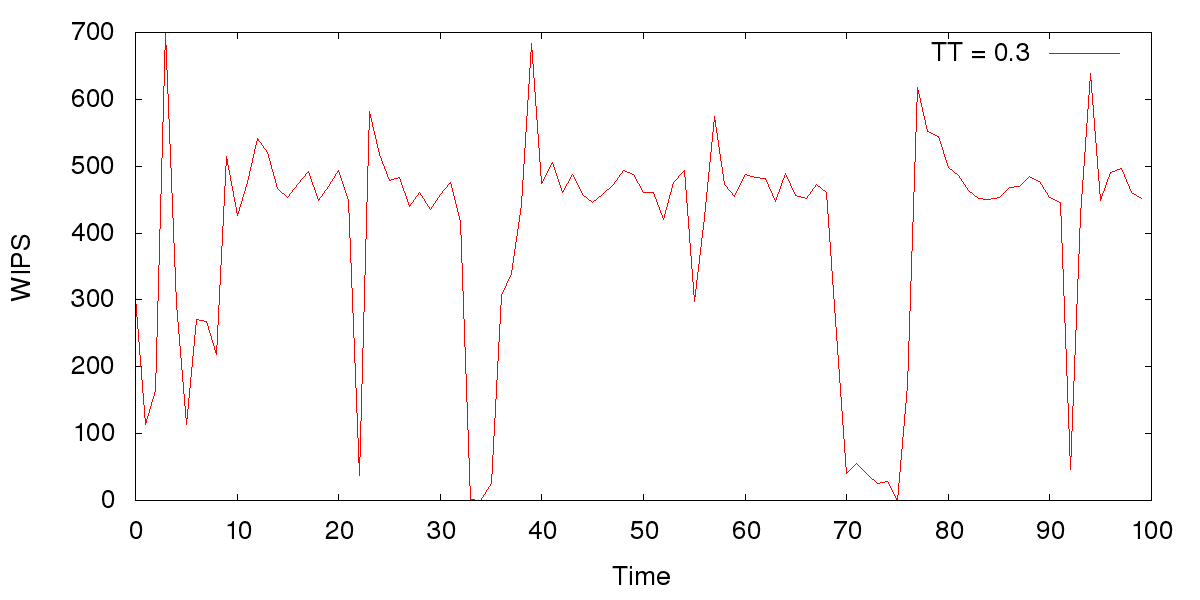
\includegraphics[width=15cm, height=10cm]{images/completo/plot_ordering_TT03.png}
Figura 13: WIPSo por tempo(s) para Think-Time de 0.3s testado no perfil de Ordering no experimento completo
\end{center}

Por fim, a primeira falha ocorreu perto de 31s e a recuperação em 40s. A segunda falha ocorreu em torno de 69s e o sistema se recuperou em torno de 77s. Logo, o tempo inoperante ficou em torno de 17s e o tempo operante em 83s, o que nos da uma disponibilidade de 83\%. 

Segue na Tabela 5 as disponibilidades obtidas.

        \begin{center}
        \begin{tabular} { | c | c |}
        \hline
        Perfil  & Disponibilidade \\ \hline
        WIPSb & 76\% \\ \hline
        WIPS & 79\% \\ \hline
        WIPSo & 83\% \\
        \hline
        \end{tabular}
        %\caption{\label{tab:tableOne}Configurações das máquinas remotas}

        Tabela 5: Disponibilidades do experimento final (1000 clientes, Think-Time = 0.3s)
    \end{center}

\section{Conclus\~ao}
Concluímos que os experimentos foram bem sucedidos.

Os experimentos um e dois, conseguiram prever com certa precisão a melhor carga a ser utilizada no experimento três, de cerca de 3000 clientes, que equivale aproximadamente ao uso de 1000 clientes com Think-Time de 0.3s.

O experimento três teve bastante sucesso nos perfis de browsing e shopping, onde a falha não fez cair o número de WIPS do servidor, pois a troca de banco de dados foi quase que imediata. Já no perfil de ordering, houve por volta de quatro segundos de tempo de recuperação para o servidor voltar a responder requisições, o que consideramos um tempo bastante razoável.

Por fim, o experimento completo foi um sucesso. Nosso sistema conseguiu se recuperar adequadamente e apresentou uma disponibilidade boa, considerando que temos apenas um banco de dados em hot-standby e não tínhamos conhecimento sobre as ferramentas utilizadas ao iniciar o projeto.

\bibliography{bib/relatorioGrupo06}{}
\bibliographystyle{ieeetr}

\end{document}
